\chapter{Category Theory}

\let\thefootnote\relax\footnote{Parts of this chapter are based on previous research done by the author and appears in his Master's Thesis \cite{ArtMestrado}}

In this chapter, we introduce the theory that we are going to use to develop the mathematical aspect of computational paths. The theory used to construct this mathematical model will be category theory. We are going to see that this theory is extremely powerful, but it is abstract and complex. With that in mind, we start this chapter defining and exposing the main basic concepts of this theory. We then use those basic concepts to arrive at more complicated results, which will be necessary in the construction of our mathematical model for computational paths. Since this model has many details and peculiarities, we leave it to the next chapter of this work. 

Category theory appeared for the first time in the works of  Eilenberg \& Mac Lane in 1945. It was originally proposed as just a tool to study natural transformations and functors\cite{Stanford7}. Functors and natural transformations are basically entities that transform one mathematical structure into another. For instance, one can transform a function between sets into a homotopy between topological spaces. Despite being proposed as only a tool, category theory grew quickly and became a well-established theory. Today, it is widely used in mathematics and computer science. Even logic and $\lambda$-calculus can be modeled by category theory. It also has been used as foundation of mathematics in place of $ZFC$ \cite{Stanford7}.

Despite its power of abstraction, category theory does not hinder the importance of type theory. It can be used as a foundation for mathematics, but it shares some problems that appears in ZFC, such as the fact that it is hard to be modeled by computers. Thus, the importance of category theory to this work is limited to the fact that it is closely related to type theory. This fact is clear when one realizes that many type theoretical constructions can be mathematically modeled using category theory.

It is also important to note that this chapter is not limited to basic category theory. To obtain the results that we want about computational paths, one also needs to define some basic concepts of higher category theory. Thus, we are going to introduce those concepts in the end of this chapter.

\section{Basic Concepts}

Category theory has a rather interesting aspect when compared directly with set theory or type theory. It is the fact that set theory and type theory have a fundamental concept in the core of those theories. One gains nothing asking what is the exact definition of sets or types, but one can ask what results can be obtained from those concepts. In category theory, this does not happen. It is possible to prove from rules and well-established entities whether some structure is a category or not. Perhaps the best way of introducing category theory is to analyze some aspects of functions. The reason for that is that one can affirm that a category is constructed based on structures called morphisms that are very similar to functions. 

Consider that we have sets $A$, $B$ and $C$ and functions $f$ and $g$ such that $f: A \rightarrow B$ and  $g: B \rightarrow C$. Thus, it is possible to construct a composite function $(g \circ f): A \rightarrow C$ defined by $(g \circ f) = g(f(x))$. We have the following diagram:
\bigskip

\begin{large}
\begin{center}
\begin{tikzcd}
A \arrow{r}{f} \arrow{rd}[swap]{g \circ f}
&B \arrow{d}{g}\\
&C
\end{tikzcd}\end{center}\end{large}

\bigskip

One should become acquainted with those kinds of diagrams, since they commonly appear in category theory. Categories are based on objects (in the above diagrams, the objects are sets) and arrows or morphisms (in the above diagram, the functions). Thus, it is natural to think that those structures are represented by diagrams. They are not just a graphic representation of some structure, since they are frequently used as the main argument in proofs of important properties.  

One interesting property rises from function composition: it is associative. In other words, if there is some $h: C \rightarrow D$, then $(h \circ g) \circ f = h \circ (g \circ f)$. This property is represented by the following diagram \cite{Steve2}:

\bigskip

\begin{large}
\begin{center}
\begin{tikzcd}
A \arrow{r}{f} \arrow{rd}[swap]{g \circ f}
&B \arrow{d}{g} \arrow{rd}{h \circ g}\\
&C \arrow{r}{h}
&D
\end{tikzcd}
\end{center}
\end{large}

\bigskip

Functions have another interesting property. For any set $A$, there is a identity function $1_{A}: A \rightarrow A$ defined by $1_{A}(a) = a$. This function can be considered as the neutral element of the composition operation, i.e. $1_{B} \circ f = f = f \circ 1_{A}$. In the next subsection we give a formal definition for the concept of category, which will give general versions of those properties.

\subsection{Categories}

Category is the main concept of category theory. Its definition follows: 

\begin{mydefi}[Categories \cite{Steve2}] A category \textbf{C} is a structure with the following elements and rules:
\begin{itemize}

\item Objects: Objects are usually represented by capital letters $A, B, C...$. The class of all objects is called $C_{0}$.

\item Arrows(morphisms): Arrows or morphisms are commonly represented by letters which are used to represent functions, such as $f, g, h...$. It is importance to notice that arrows always appear between two objects. The class of all arrows is called $C_{1}$.

\item Domain and range: Given any arrow  $f: A \rightarrow B$, the domain of $f$ is $A$ and is written as  $dom(f) = A$. The range of $f$ is $B$ and is written as $cod(f) = B$. 

\item Composition: Given any arrows  $f: A \rightarrow B$ and $g: B \rightarrow C$, there is always an arrow $h = (g \circ f): A \rightarrow C$. This arrow is the composition of $f$ and $g$. Moreover, $h$ has a universal property, i.e., given any $m = (g \circ f)$, then $m = h$. 

\item Identity Arrow: For any object $A$ there is an arrow  $1_{A}: A \rightarrow A$ called identity arrow.

\item Associativity rule: Given any arrows $f: A \rightarrow B$, $g: B \rightarrow C$ and $h: C \rightarrow D$, then $(h \circ g) \circ f = h \circ (g \circ f)$ always holds.

\item Identity rule: Given any $f: A \rightarrow B$, then $1_{B} \circ f = f = f \circ 1_{A}$.

\end{itemize}

\end{mydefi}

From the above definition, it is clear that a function has a categorical structure. In fact, one of the most common category is \textbf{Sets}. In this category, objects are sets and arrows are functions between sets. As we have just seen, a function follows associative and identity rules and thus, \textbf{Sets} is clearly a category. Before we define further concepts, it is important to show the use of the above definition in another example. An interesting one is the structure \textbf{Pos}. As we have seen in \emph{chapter 1}, a set can be ordered by an order relation $\leq$. Those ordered sets are known as \emph{posets} (partially ordered sets). That way, an object in this structure is a poset and an arrow is a monotone function \cite{Steve2}. A function is monotone iff $a \leq b \Rightarrow f(a) \leq f(b)$.

\begin{prop} \textbf{Pos} is a category.
\end{prop}

\begin{proof}
	
A proof that some structure is a category follows a well-defined set of steps. Initially, it is necessary to define what is an arrow, the compositions and the identity arrow. Then, one just needs to check if the rules of associativity and identity hold.

\begin{itemize}

\item Composition: The composition is similar to the one given in \textbf{Sets}, i.e., given any $f: A \rightarrow B$ and $g: B \rightarrow C$,  then one can define  $(g \circ f) = g(f(x))$. In the case of \textbf{Pos}, $(g \circ f)$ needs to be monotone. Suppose that $a \leq b$. Since $f$ is monotone, then $f(a) \leq f(b)$. Since $g$ is monotone, then  $g(f(a)) \leq g(f(b))$ and thus, $g \circ f$ is monotone.  

\item Identity: The identity arrow will also be similar to the one in \textbf{Sets}, i.e., the identity arrow will be an $1_{A}: A \rightarrow A$ defined by $1_{A}(a) = a$.  $1_{A}$ is clearly monotone, since $a \leq b$ then  $1_{A}(a) = a \leq b = 1_{A}(b)$.  

\item Associativity rule: Since arrows are functions, the associative rule clearly holds.

\item Identity rule: Analogous to the associative rule. It has already proved for functions that $1_{A}$ respects the identity rule.
\end{itemize}
\end{proof}

Therefore \textbf{Pos} is a category. Our choice of \textbf{Pos} as an example was intentional, since it is a category of great importance to computer science. The reason for that is the fact that \textbf{Pos} is used on the formalization of boolean algebra. Nevertheless, this formalization is out of the scope of this work. After introducing the concept of category, we can proceed with other interesting concepts.

\subsection{Isomorphism}

In many areas of mathematics it is rather common to work with two different structures that have similar properties. Sometimes one wants to establish a direction connection between those structures. To do this, one establishes an isomorphism. The main problem is that the definition of isomorphism is intrinsically dependent to the structure being used. For example, the concept of isomorphism between sets is different to isomorphism between posets, which is different from an isomorphism between groups. Thus, the unification of those different definitions for the same concept would be a great feat. Fortunately, this can be easily done in category theory. It also showcases how powerful is this theory. We have the following definition:  

\begin{mydefi}[Isomorphism \cite{Steve2}]: In a category \textbf{C}, an arrow $f: A \rightarrow B$ is called isomorphism if there exists an arrow  $g: B \rightarrow C$ such that  $g \circ f = 1_{A}$ and  $f \circ g = 1_{B}$. When this happens, $g$ is called inverse of $f$. We say that $A$ is isomorphic to $b$ and the write $A \cong B$. The arrow that generated this isomorphism is written as: $f: A \xrightarrow{\sim} B$.
	
\end{mydefi}

\begin{prop} Given any isomorphism $f$ and a inverse $g$ of $f$, then $g$ is unique.
\end{prop}

\begin{proof}

Let h be an inverse of $f$ To show that $g$ is unique, one needs to show that $h = g$. The following equations establish this result:

\begin{center}
$(g \circ f) \circ h = g \circ (f \circ h)$ \\
$1_{A} \circ h = g \circ 1_{B}$\\
$h = g$.
\end{center}

One can see that the first equation comes directly from the associativity of the composition. The second comes from the fact that $g$ and $h$ are inverses of $f$. The last equation comes from the fact that composition respects the identity rule. 
\end{proof}

Using the above result we can create a notation for an inverse of an isomorphism $f$. Since an inverse $g$ is unique, we can write it as $f^{-1}$.

Using this definition, what would constitute an isomorphism in \textbf{Sets}? One can notice that sets $A$ and $B$ are isomorphic iff there is a  $f: A \rightarrow B$ and a $g: B \rightarrow A$ such that $g(f(x)) = x$. Thus, $g = f^{-1}$, i.e., $g$ is the inverse of $f$. In set theory, a function has an inverse iff $f$ is bijective. Thus, $A$ and $B$ are isomorphic in \textbf{Sets} iff there is an injective function $f$ from $A$ onto $B$. Some interesting results arise from this definition of isomorphism:   

\begin{prop} $A$ and $B$ are isomorphic in \textbf{Sets} iff they have the same cardinality (this result can be informally interpreted as both sets having the same size).
\end{prop}

\begin{proof}
One can prove directly both sides of this proof. In one hand, One knows that if $A$ and $B$ are isomorphic, then there is a bijection $f: A \rightarrow B$. Since two sets by definition have the same cardinality if there is a bijection between them, then $A$ and $B$ have the same cardinality. On the other hand, if two sets have the same cardinality then there exists a bijection $f$ between them, Thus, they are isomorphic.
\end{proof}

In set theory, it is well known that one can prove that $\mathbb N$, $\mathbb Z$ e $\mathbb Q$ have the same cardinality \cite{introSet}. Thus, by the above proposition, the naturals are isomorphic to the integers and to the rationals. At a first glance, it can be completely counterintuitive. The naturals have the same structure as the integers? To answer this, one should remember that in \textbf{Sets} the object of the category is only a set. Thus, this category does not consider a set together with a order relation. If one considers the naturals and integers with their usual orderings, then it is obvious that they are not isomorphic. One direct argument is that in their usual orderings, the naturals are well-ordered, but the integers are not.

What would constitute an isomorphism in \textbf{Pos}? Given two orderings $(A, \leq')$ and $(B, \leq'')$, one can think of an isomorphism as a bijection $f$ between $A$ and $B$ that respects the ordering, i.e., if $a, b \in A$ and $a \leq' b$, then $f(a) \leq'' f(b)$.

From this definition of isomorphism, one can show that one can pick a suitable ordering to make the naturals isomorphic to the integers: 

\begin{proof}

Consider the naturals together with its traditional ordering, i.e,  $(\mathbb N, \leq) = {0,1,2,...}$. For the integers, consider an ordering $\leq''$ such that $(\mathbb Z, \leq'') = {0,-1,1,-2,2,-3,3....}$. One needs to find a bijection $f$ such that $f(0) = 0$, $f(1) = -1$, $f(2) = 1$, $f(3) = -2$, etc. To do that, one can define  $f(x) = (-1)^{x}. \ceil*[\big]{\frac{x}{2}}$. $f$ is clearly monotone, i.e.,  $a \leq b \Rightarrow f(a) \leq'' f(b)$ and it is also onto. Thus,  $(\mathbb N, \leq) \cong (\mathbb Z, \leq'')$.
\end{proof}

In this subsection, we have seen a way of using category theory to give a general definition for a important concept of mathematics. We have also shown practical examples using \textbf{Sets} and \textbf{Pos}. Isomorphism will be an essential concept in the mathematical model of computational paths.

\subsection{Groupoid}

We can use the concept of isomorphism to define a structure known as groupoid. It has the following definition: 

\begin{mydefi}[Groupoid \cite{Steve2}] Given any category \textbf{C}, we say that \textbf{C} is a groupoid iff every arrow $f \in C_{1}$ is an isomorphism. In other words, every pair of objects are mutually isomorphic. 
\end{mydefi}

The concept of groupoid plays a main role in the semantical definition of the identity type. If a category \textbf{C} is a groupoid, then every object of \textbf{C} has a similar structure. In fact, this concept has achieved great importance due to the discovery of the fact that types in Martin-L\"of's type theory have a groupoid structure \cite{hofmann1}. In fact, one can prove that types have a weak groupoid structure. Weak here means that the equalities do not hold on the nose (i.e., the equalities are not definitional), but only up to propositional equality. One will have a better grasp of the concept of a weak structure in the next chapter, when we introduce the weak groupoid model of computational paths. In fact, one of the objectives of our next chapter is to show that one can use computational paths to build a weak structure similar to the one proposed by \cite{hofmann1}, which uses the usual formulation of the intensional identity type to build it. With that in mind, one should notice that groupoid plays an important rule in this work. 

We leave further details of this topic for the next chapter. Nevertheless, to better illustrate this concept, we are going to give simple examples. Take a category whose objects are sets and the arrows are bijections between these sets. Since bijections are isomorphisms, this category constitutes a groupoid structure. Another example of groupoid is constructed using \textbf{Pos}. One can take a category whose objects are ordered sets $(A_{n}, \leq _{n})$ and arrows are bijections that respect the orderings. Thus, every arrow is an isomorphism.

\subsection{Functors}

The notion of functor is one of the most interesting and important concepts of category theory. Functors could be understood as a function that receives a category as input. Therefore, a functor transforms one category into another For example, one could think of the transformation of a category \textbf{C} into a category \textbf{D}. To do that, one needs to transform every object of \textbf{C} into a object of \textbf{D} and the arrows of \textbf{C} into arrows of \textbf{D}. Moreover, the associativity and identity rule must be preserved. We have the following formal definition: 

\begin{mydefi}[Functor \cite{Steve2}] A functor $F: \textbf{C} \rightarrow \textbf{D}$ between categories \textbf{C} and \textbf{D} is a mapping of objects and arrows such that:

\begin{itemize}

\item $A \in C_{0}$ is mapped to $F(A) \in D_{0}$,

\item $f: A \rightarrow B \in C_{1}$ is mapped to $F(f): F(A) \rightarrow F(B) \in D_{1}$,

\item $F(g \circ f) = F(g) \circ F(f)$,

\item $F(1_{A}) = 1_{F(A)}$.

\end{itemize}
\end{mydefi}

Perhaps a better way of understanding the above definition is to visualize it through the help of diagrams \cite{Steve3abnt}:

\begin{example} \normalfont This example is going to show the diagram representation of the action of a generic functor  $F: \textbf{C} \rightarrow \textbf{D}$. Let \textbf{C} be a category represented by the following diagram: 

\bigskip

\begin{large}
\begin{center}
\begin{tikzcd}
A \arrow [loop left]{l}{1_{A}} \arrow{r}{f} \arrow{rd}[swap]{g \circ f}
&B \arrow{d}{g}\\
&C
\end{tikzcd}\end{center}\end{large}

\bigskip

After applying a functor $F$, one ends up with $F(\textbf{C}) = \textbf{D}$. This is represented by the following diagram: 

\bigskip

\begin{large}
\begin{center}
\begin{tikzcd}
F(A) \arrow [loop left]{l}{F(1_{A}) = 1_{F(A)}} \arrow{r}{F(f)} \arrow{rd}[swap]{F(g \circ f) = F(g) \circ F(f)}
&F(B) \arrow{d}{F(g)}\\
&F(C)
\end{tikzcd}\end{center}\end{large}

\end{example}

\bigskip

Functors are common in practice. A simple example is the functor $For: \textbf{Pos} \rightarrow \textbf{Sets}$. One can define $For$ explaining its action on the objects and arrows of \textbf{Pos}. As we have seen, an object of \textbf{Pos} is a pair $(A,\leq)$, in which $A$ is a set. $For$ has the following behavior: $For(A,\leq) = A$. In the arrows, we have that $For(f: (A,\leq) \rightarrow (B,\leq ')) = f: A \rightarrow B$. Thus, $For$ can be seen as a forgetful functor that forgets the ordering of a ordered set, returning only the set. For the arrows, $For$ forgets that $f$ is a monotone function, returning only the function. Forgetful functors are common in mathematics. Another well known example is $For: \textbf{Grp} \rightarrow \textbf{Sets}$. This functor receives a category of groups as input. It then forgets the group structure, returning only the underlying set. Forgetful functors plays a fundamental role in category theory, since it is the basic concept behind the concept of adjoint.  

Further in this chapter we are going to see that the use of functors is needed in the definition of a $2$-category.


\subsection{Duality}

Duality is a principle of category theory that states that for any category \textbf{C}, there is a dual category \textbf{$C^{OP}$}. This category is defined in the following way \cite{Steve3abnt}:

\begin{mydefi} Given any category \textbf{C}, the category $\textbf{C}^{OP}$ is the dual category of \textbf{C} and is defined in the following way::

\begin{itemize}

\item $\textbf{C}_{0}^{OP} =  \textbf{C}_{0}$.
\item $\textbf{C}_{1}^{OP} =  \textbf{C}_{1}$.
\item $dom$ $\textbf{C}^{OP}$ = $cod$ \textbf{C}.
\item $cod$ $\textbf{C}^{OP}$ = $dom$ \textbf{C}.
\end{itemize}

\end{mydefi}

We can represent this duality using diagrams. Given any category \textbf{C} represented by the following diagram:

\bigskip

\begin{large}
\begin{center}
\begin{tikzcd}
A  \arrow [loop left]{l}{1_{A}} \arrow{r}{f} \arrow{rd}[swap]{g \circ f}
&B \arrow{d}{g}\\
&C
\end{tikzcd}\end{center}\end{large}

\bigskip

Thus,  \textbf{$C^{OP}$} is given by:

\bigskip

\begin{large}
\begin{center}
\begin{tikzcd}
A  \arrow [loop left]{l}{\bar{1_{A}} = 1_{A}}
&B \arrow{l}[swap]{\bar{f}}\\
&C \arrow{u}[swap]{\bar{g}} \arrow{lu}{\bar{g \circ f} = \bar{f} \circ \bar{g}}
\end{tikzcd}\end{center}\end{large}

\bigskip

From a dual category, one can define a new kind of functor known as contravariant functor. A contravariant functor is given by $F: \textbf{C}^{OP} \rightarrow \textbf{D}$. Instead of defining a functor that acts on a category  $\textbf{C}^{OP}$, one can apply directly a contravariant functor in a category \textbf{C}. To do that, one just needs to invert the order of the arrows in the application of the functor. To better see this, consider \textbf{C} as the category of the above example. We have the following diagram of an application of a contravariant functor $F$:

\bigskip

\begin{large}
\begin{center}
\begin{tikzcd}
A  \arrow [loop left]{l}{F(1_{A)}}
&B \arrow{l}[swap]{F(f)}\\
&C \arrow{u}[swap]{F(g)} \arrow{lu}{F(g \circ f)}
\end{tikzcd}\end{center}\end{large}

\bigskip

The use of contravariant functors in category theory is common. Also, duality is a very useful principle, since many properties of category theory appears from the dual category of some property. For example, if one has a diagram that represents the product of two categories, one just needs to get the dual category to define the coproduct. 

\subsection{Commutativity}

In this subsection, we introduce two kinds of diagrams widely used in category theory, the commutative triangle and commutative square. 

\begin{mydefi}[Commutative triangle] A commutative triangle is the following diagram: 
\bigskip

\begin{large}
\begin{center}
\begin{tikzcd}
A \arrow{r}{f} \arrow{rd}[swap]{h}
&B \arrow{d}{g}\\
&C
\end{tikzcd}
\end{center}
\end{large}

\bigskip

Since it commutes, the triangle $ABC$ respects the following equation: $g \circ f = h$.

\end{mydefi}

\begin{mydefi}[Commutative square] A commutative square is the following diagram:
	
\bigskip

\begin{large}
\begin{center}
\begin{tikzcd}
A \arrow{r}{f} \arrow{d}{t}
&B \arrow{d}{g}\\
C \arrow {r}{s}
&D
\end{tikzcd}
\end{center}
\end{large}

\bigskip

Since it commutes, the square $ABCD$ respects the following equation: $g \circ f = s \circ t$.

\end{mydefi}

Those two diagrams are used to define and prove many entities and properties of category theory.

\subsection{Product between two categories}

Before we define product between two categories, it is important to notice that there is a significant difference between product between categories and product between objects of a category. Product between categories is an operation that builds another category, whereas a product between objects of a category builds another object. Moreover, we can always obtain the product of two categories, but sometimes the product of two objects does not exist. Thus, in this subsection we introduce the product between two categories. We are also going to introduce the product between two objects in the sequel, since it is directly connected to the product of two types in type theory.

\begin{mydefi}[Product between two categories \cite{Steve2}] Given any categories \textbf{C} and \textbf{D}, one can obtain a category \textbf{C $\times$ D} defined by:

\begin{itemize}

\item Objects: Objects have the form $(C,D)$, with $C \in C_{0}$ e $D \in D_{0}$.
\item Arrows: Arrows have the form $(f,g): (C,D) \rightarrow (C',D')$, with $f: C \rightarrow C' \in C_{1}$ e $g: D \rightarrow D' \in D_{1}$.
\item Composition: Composition is defined component-wise, given by  $(f',g') \circ (f,g) = (f' \circ f,g' \circ g)$.
\item Identity: The identity arrow is also defined component-wise, given by $1_{(C,D)} = (1_{C}, 1_{D})$. 

\item Two projection functors, represented by the following diagram:

\bigskip

\begin{large}
\begin{center}
\begin{tikzcd}
\textbf{C}
&\textbf{C} \times \textbf{D} \arrow{l}[swap]{\pi_{1}} \arrow{r}{\pi_{2}}
&\textbf{D}
\end{tikzcd}\end{center}\end{large}

\bigskip

The projections respects the following equations: 
\begin{center}
	$\pi_{1}(C,D) = C$ \quad $\pi_{2}(C,D) = D$ \\ 
	$\pi_{1}(f,g) = f$ \quad $\pi_{2}(f,g) = g$.

\end{center}

\end{itemize}
\end{mydefi}

This definition will play an important role in the definition of bicategory, as we are going to see further in this chapter.

\subsection{Hom and Small Categories}

In category theory, there is a important structure called $Hom$ and defined as: 

\begin{mydefi}[$Hom_{\textbf{C}}(A,B)$ \cite{Steve3abnt}] $Hom_{\textbf{C}}(A,B)$ is a structure that contains all arrows from object $A$ to object $B$, both objects of \textbf{C}.
\end{mydefi}

Why we called $Hom$ a structure instead of a set? The reason for that is the fact that sometimes $Hom$ is more than just a set. In higher categories, for example, $Hom$ can be a category. Also, when we talk about the size of a category, one has the following definitions: 

\begin{mydefi}[Large and small category \cite{Steve2}] A category \textbf{C} is called small if $C_{0}$ and $C_{1}$ are sets. Otherwise the category is called large.
\end{mydefi}

The concept of large category rose up from the fact that in many categories the objects and arrows cannot be represented by sets. In many cases, each object of a category is another category. The same thing can happen to the arrows. Moreover, another important thing to notice is that many properties are only valid in small categories. This happens because some properties are directly dependent on the fact that the objects and arrows are sets. We have one more relevant definition: 

\begin{mydefi}[Locally small category \cite{Steve2}] A category \textbf{C} is locally small if for any pair of objects $A, B \in C_{0}$, then $Hom_{\textbf{C}}(A,B)$ is a set. 
\end{mydefi}

Sometimes we just need some category \textbf{C} to be locally small. This will become more clear further in this chapter, when we investigate some properties of higher categories. 

\section{Product in a Category}

In the previous section, we have seen the definition of product between categories. In this section, our objective is to define product between objects of a category. This plays an important role in this work, since it has a direct connection with product of types, as we are going to show in this section. Based on those connections that we have decided to use category theory to propose a mathematical model for computational paths, as we are going to do in the next chapter.

\begin{mydefi}[Product in a category \cite{nlabProductabnt}] In a category \textbf{C}, the product between two objects $X,Y \in C_{0}$ is an object $X \times Y$ equipped with morphisms $p: X \times Y \rightarrow X$ and $q: X \times Y \rightarrow Y$, which are called projections. Moreover, the product has a universal property, which states that given any $Z \in C_{0}$ and maps $f: Z \rightarrow X$ and $g \rightarrow Z \rightarrow Y$, then there exists a unique map $h: Z \rightarrow X \times Y$ such that $p \circ h = f$ and $q \circ h = g$.  
\end{mydefi}

This is represented in the following diagram \cite{Steve2}:

\bigskip

\begin{large}
\begin{center}
\begin{tikzcd}
&Z \arrow {dl}[swap]{f}  \arrow[dotted]{d}{h} \arrow{rd}{g} \\
X
&X \times Y \arrow{l}{p} \arrow{r}[swap]{q}
&Y
\end{tikzcd}\end{center}\end{large}

\bigskip

In the above diagram, the triangles are commutative. If one pays attention to the definition, the projections are easy to understand. Nevertheless, the part that related to the universal property, i.e., $Z$ and the unicity of $h$ might be a little complicated. This part can be explained in the following way: If there is an arrow $f: Z \rightarrow X$  and  $g: Z \rightarrow Y$, then the unicity of $h: Z \rightarrow X \times Y$ indicates that there is only one way to construct the product from these two arrows. Therefore, we can write $h$ uniquely as $h = (f,g)$.  


\begin{prop} In \textbf{Sets}, the product between two objects $A,B \in Sets_{0}$ is the cartesian product between two sets.
\end{prop}

\begin{proof}
To show that the product between two sets is the cartesian product, the first thing one needs to do is to show the projects. Thus, one just needs to define $p: A \times B \rightarrow A$ as $p(a,b) = a$ and define $q: A \times B \rightarrow B$ as $q(a,b) = b$. Now, one needs to show the universal property. Let  $f: Z \rightarrow A$ and $g : Z \rightarrow B$. One can define a $h: Z \rightarrow A \times B$ in the following way: $h(x) = (f(x),g(x))$. To end this proof, one needs to check that $p \circ h =f$ and $q \circ h = g$. Indeed, $(p \circ h)(x) = p(h(x)) = p(f(x),g(x)) = f(x)$. Analogously, $(q \circ h)(x) = q(h(x)) = q(f(x),g(x)) = g(x)$. Therefore, the cartesian product of two sets should be seen a the product between two objects of \textbf{Sets}.
\end{proof}

A natural questions arises. Is it possible to find another definition for the product of two objects in \textbf{Sets}. The following proposition answers this question \cite{Steve2}:

\begin{prop}
If $\times$ and $\times '$ are products of a category \textbf{C}, then $A \times B \cong A \times ' B$.
\end{prop}

\begin{proof}

This is one case that the a proof with the help of diagrams is much easier to see \cite{Steve2}:

\bigskip

\begin{large}
\begin{center}
\begin{tikzcd}
&A \times B \arrow {dl}[swap]{p_{1}}  \arrow[dotted]{d}{(p_{1},p_{2})} \arrow{rd}{p_{2}} \\
A
&A \times ' B \arrow{l}{q_{1}}  \arrow[dotted]{d}{(q_{1},q_{2})}  \arrow{r}[swap]{q_{2}}
&B\\
&A \times B \arrow {ul}{p_{1}} \arrow{ru}[swap]{p_{2}}

\end{tikzcd}\end{center}\end{large}

\bigskip

The main point here is that from the universal property of the products, one can obtain the arrows $(p_{1},p_{2})$ and $(q_{1},q_{2})$. Moreover, all triangles in the above diagram are commutative. Looking at the diagram, the following equations are obtained from the triangles $(A \times B)(A \times B)A$ and $(A \times B)(A \times B)B$: 

\begin{center}
$p_{1} \circ (q_{1},q_{2}) \circ (p_{1},p_{2}) = p_{1}$

$p_{2} \circ (q_{1},q_{2}) \circ (p_{1},p_{2}) = p_{2}$
\end{center}


Indeed, $(q_{1},q_{2}) \circ (p_{1},p_{2})$ acts as the identity arrow of $A \times B$. By the unicity of those arrows, one knowns that $(q_{1},q_{2}) \circ (p_{1},p_{2}) = 1_{A \times B}$. Using the symmetry of the diagram, one obtains $(p_{1},p_{2}) \circ (q_{1},q_{2})   = 1_{A \times ' B}$. Therefore $ (p_{1},p_{2})$ and  $(q_{1},q_{2})$ are inverses and establish the isomorphism between the two products.
\end{proof}

Based on this proof, it is possible to state that every category has only one definition for the product of two objects since all possible definitions are mutually isomorphic.

\subsection{Product in Type Theory and Category Theory}

This section is going to show the close relation between type theory and category theory. To see that, we are going to show some type theoretic constructions together with the respective diagrams in type theory. We start with \gls{pf} \cite{nlabProductabnt}:

\bigskip

\begin{equation*}
\begin{bprooftree}
\AxiomC{$A$ type}
\AxiomC{$B$ type}
\RightLabel{$\times - F$}
\BinaryInfC{$A \times B$ type}
\end{bprooftree}
\end{equation*}

\bigskip

Product formation is intuitive. Given any types $A$ and $B$, it is possible to obtain $A \times B$. In categories, there is an equivalent proposition: If $A, B \in C_{0}$, then $A \times B in C_{0}$. Now we have \gls{pi} \cite{nlabProductabnt}:

\bigskip

\begin{equation*}
\begin{bprooftree}
\AxiomC{$a : A$}
\AxiomC{$b : B$}
\RightLabel{$\times - I$}
\BinaryInfC{$\langle a,b\rangle: A \times B$}
\end{bprooftree}
\quad
\begin{large}
\begin{tikzcd}
&Z \arrow {dl}[swap]{a}  \arrow[dotted]{d}{(a,b)} \arrow{rd}{b} \\
A
&A \times B
&B
\end{tikzcd}
\end{large}
\end{equation*}

\bigskip

Indeed, given any terms $a : A$ and $b : B$, it is possible to construct  $\langle a,b\rangle : A \times B$. In categories, it is represented by arrows $a$ and $b$. Given those arrows, it is possible to obtain a unique $\langle a,b\rangle$ given by the universal property of the product. Now follows the \gls{pe1} and the \gls{pe2} \cite{nlabProductabnt}:

\bigskip

\begin{equation*}
\begin{bprooftree}
\AxiomC{$t : A \times B$}
\RightLabel{$\times - E_{1}$}
\UnaryInfC{$p_{1}(t): A$}
\end{bprooftree}
\quad
\begin{bprooftree}
\AxiomC{$t : A \times B$}
\RightLabel{$\times - E_{2}$}
\UnaryInfC{$p_{2}(t): B$}
\end{bprooftree}
\quad
\begin{large}
\begin{tikzcd}
&Z \arrow[dotted]{d}{t} \\
A
&A \times B \arrow{l}[swap]{p_{1}} \arrow{r}{p_{2}}
&B
\end{tikzcd}
\end{large}
\end{equation*}

\bigskip

The eliminations are done using the projections. This is exactly that the above diagram represents. We also have diagram representations of the computation rules $p_{1}(\langle a,b\rangle) = a$ and $p_{2}(\langle a,b\rangle) = b$:

\bigskip

\begin{equation*}
\begin{large}
\begin{tikzcd}
&Z \arrow {dl}[swap]{a}  \arrow[dotted]{d}{\langle a,b\rangle} \arrow{rd}{b} \\
A
&A \times B \arrow{l}[swap]{p_{1}} \arrow{r}{p_{2}}
&B
\end{tikzcd}
\end{large}
\end{equation*}

\bigskip

That way, one can see that we can translate type theoretic constructions to the language of category theory. In this subsection, we have shown the specific case of the product, but using a similar process one can translate any entity of type theory, including path-induction and the constructor $J$.

\subsection{Coproduct}

The objective of this section is not to give a detailed construction of the coproduct, but to show that it is possible to use duality on the constructions of the product to obtain direct constructions of the coproduct. Given any a category \textbf{C} and objects $A,B \in C_{0}$, the coproduct of two objects is represented by $A + B$ and given by the following diagram:

\bigskip

\begin{equation*}
\begin{large}
\begin{tikzcd}
&Z  \\
'A \arrow{ru}{f} \arrow{r}[swap]{i_{1}}
&A + B \arrow[dotted]{u}[swap]{[a,b]}
&B \arrow {lu}[swap]{g} \arrow{l}{i_{2}}
\end{tikzcd}
\end{large}
\end{equation*}

\bigskip

As one can see, the coproduct is exactly the dual category of the product. The projections are replaced by injections. It also has a universal product, that states the following: if there are $f: A \rightarrow Z$ and $g: B \rightarrow Z$, then there is a unique $h: A + B \rightarrow Z$. We can also use duality to prove the following proposition:

\begin{prop}
If $+$ and $+ '$ are coproducts of a category \textbf{C}, then $A + B \cong A +' B$. 
\end{prop}

\begin{proof}
The proof is directly connected to the fact that the dual of an isomorphism is also an isomorphism. The duality only changes the direction of the arrow. Thus, if an arrow is an isomorphism in the original category, then it will also be in the dual. Since the isomorphism has been proved for the product, the duality keeps it
\end{proof}

Using the same process that we have established for the product, one can translate the construction of the coproduct in type theory to the language of category theory.

\section{Natural Transformations}

Natural transformations are one of the most important concepts of category theory. As we have said in the introduction of this chapter, category theory was originally proposed to study natural transformations. Moreover, we are going to use this concept in the definition of bicategory. Perhaps a good way of introducing natural transformations is the following example: Suppose that $A, B$ and $C$ are objects of a category with products. Then,  $(A \times B) \times C \cong A \times (B \times C)$ \cite{Steve2}. We will not show the proof of this proposition, since it is pretty straightforward. One just needs to draw the diagram and establishes the equations using the commutative triangles. Nevertheless, the important piece o information is the fact that there exists an isomorphism  $f: (A \times B) \times C \xrightarrow{\sim} A \times (B \times C)$.   This isomorphism $f$ has a limitation though. It establishes only the isomorphism for objects $A, B$ and $C$. Ideally, one wants a general result that does not depend on the choice of objects $A, B$ or $C$. To do that, one needs the concept of natural transformations.

Intuitively, a natural transformation is a morphism between functors. We can use the associativity of the product as our first example of natural transformation. First, one can conceive the following functors:  $F: \textbf{C} \times \textbf{C}\times \textbf{C} \rightarrow \textbf{C}$ defined by  $F = (-_{1} \times -_{2}) \times -_{3}$ and the functor $G: \textbf{C} \times \textbf{C} \times \textbf{C} \rightarrow \textbf{C}$ defined by  $G = -_{1} \times (-_{2} \times -_{3})$.    With that in mind, one needs to find a natural transformation  $\theta: F \rightarrow G$. Moreover, one also needs to show that $\theta$ is an entity known as natural isomorphism. Thus, one finishes the proof that the isomorphism  $(A \times B) \times C \cong A \times (B \times C)$ does not depend on the choice of the objects. In that case, it is said that the isomorphism is natural on $A, B$ and $C$. Here follows a formal definition for natural transformation:   

\begin{mydefi}[Natural transformation \cite{Steve2}] Given any categories \textbf{C} and \textbf{D} and functors $F,G : \textbf{C} \rightarrow \textbf{D}$, a natural transformation  $\theta: F \rightarrow G$ is a family of arrows in \textbf{D} given by:  ($\theta_{C}: FC \rightarrow GC)_{C \in C_{0}}$. Moreover, given a $f : C \rightarrow C' \in C_{1}$, then $\theta_{C'} \circ F(f) = G(f) \circ \theta_{C}$. This equality is represented by the following commutative square:   

\bigskip

\begin{large}
\begin{center}
\begin{tikzcd}
FC \arrow{r}{\theta_{C}} \arrow{d}{F(f)}
&GB \arrow{d}{G(g)}\\
FC' \arrow {r}[swap]{\theta_{C'}}
&GD
\end{tikzcd}
\end{center}
\end{large}

\bigskip

The arrows $\theta_{C}$ are called components $\theta$ in $C$.
\end{mydefi}

Looking at the above definition, one can conclude that to find a natural transformation between two functors, one just needs to find a suitable morphism for the components. This morphism needs to be natural, i.e, it must obey the commutative square. From the definition of natural transformation, one can define the following category:

\begin{mydefi}[Category $Fun(\textbf{C},\textbf{D})$ \cite{Steve2}] Given any categories \textbf{C} and \textbf{D}, it is possible to construct the category  $Fun(\textbf{C},\textbf{D})$ defined by:

\begin{itemize}

\item Objects: Objects are functors $F: \textbf{C} \rightarrow \textbf{D}$.
\item Arrows: Arrows are natural transformations $\theta : F \rightarrow G$.
\item Composition: Given any two arrows $\theta: F \rightarrow G$ e $\phi: G \rightarrow H$, it is possible to define $(\phi \circ \theta)$ component-wise: $(\phi \circ \theta)_{C} = \phi_{C} \circ \theta_{C}$.
\item Identity: Given any functor $F$, the arrow $1_{F}$ is defined component-wise: $(1_{F})_{C} = 1_{FC} : FC \rightarrow FC$.
\end{itemize}
\end{mydefi}

Therefore, we can now define natural isomorphism:

\begin{mydefi}[Natural isomorphism \cite{Steve2}] A natural isomorphism is a natural transformation  $\theta: F \rightarrow G$ such that $\theta$ is an isomorphism in the category $Fun(\textbf{C},\textbf{D})$.
\end{mydefi}

There is a easier way to check if a natural transformation is an isomorphism  \cite{Steve2}:
	
\begin{prop}
A natural transformation $\theta: F \rightarrow G$ is a natural isomorphism iff every component  $\theta_{C}: FC \rightarrow GC$ is an isomorphism.
\end{prop}

\begin{proof}

$(\Rightarrow)$ To prove this direction, one needs to prove that given any natural isomorphism  $\theta: F \rightarrow G$,, then every component $\theta_{C}$ is also an isomorphism. Since $\theta$ is an isomorphism, then $\theta$ has an inverse $\phi: G \rightarrow F$. Thus, one has that $\theta \circ \phi = 1_{G}$ and $\phi \circ \theta = 1_{F}$. Thus, if one takes any component in $C$, one concludes that  $(\theta \circ \phi)_{C} = (1_{G})_{C}$ and  $(\phi \circ \theta)_{C} = (1_{F})_{C}$. By the definition of composition and identity in $Fun$, one obtains $\phi_{C} \circ \theta_{C} = 1_{FC}$  and $\theta_{C} \circ \phi_{C} = 1_{GC}$. Therefore, $\phi_{C}$ is inverse to $\theta_{C}$. Therefore, every component is an isomorphism.

$(\Leftarrow)$ To prove the opposite direction, one needs to show that if every component $\theta_{C}$ of a natural transformation $\theta$ is an isomorphism, then $\theta$ is also an isomorphism. If each component is an isomorphism then for each $\theta_{C}$ there exists an inverse arrow  $\phi_{C}$ such that $\theta_{C} \circ \phi_{C} = 1_{GC}$ and $\phi_{C} \circ \theta_{C} = 1_{FC}$. By the definition of composition and identity of $Fun$, one has that $\theta_{C} \circ \phi_{C} =  (\theta \circ \phi)_{C} =  1_{GC} = (1_{G})_{C}$. Thus, $\theta \circ \phi = 1_{G}$. Analogously, one shows that  $\phi \circ \theta = 1_{F}$. Therefore, $\phi$ is a natural transformation inverse to $\theta$. One concludes that $\theta$ is natural isomorphism.
\end{proof}

The above proposition makes the notion of natural isomorphism easier to work with, since one only needs to show that every component is an isomorphism. To show how one can use natural transformations and natural isomorphisms in practice, consider the following proposition:

\begin{prop}
Let \textbf{C} be a category that has binary products and $A,B \in C_{0}$, then $A \times B \cong B \times A$ and the isomorphism is natural in $A$ and in $B$.
\end{prop}

If we limited the above proposition to a proof of $A \times B \cong B \times A$, then it would be a matter of showing diagrams of the product to establish this isomorphism. Nevertheless, we also need to show that this isomorphism is natural in $A$ and in $B$. There is only one way of doing that: using natural transformations. Here is the proof \cite{Steve2}:

\begin{proof}

To prove this natural isomorphism, one needs to define the functors first. The first functor is  $\times: \textbf{C} \times \textbf{C} \rightarrow \textbf{C}$, defined by $\times = (-_{1},-_{2})$. The second is given by $\bar{\times}: \textbf{C} \times \textbf{C} \rightarrow \textbf{C}$ defined by $\bar{\times}: (-_{2},-_{1})$. Thus, in objects  $A \bar{\times} B = B \times A$ and in arrows $\alpha \bar{\times} \beta = \beta \times \alpha$. that way, one now needs to conceive a natural transformation $\theta$ between those two functors. One can define $\theta$ by its behavior when applied in terms $(A,B)$. Thus, one can define $\theta_{(A,B)}(a,b) = (b,a)$, with $a$ and $b$ arrows of a product (i.e., given a $Z$, they are arrows  $Z \rightarrow A$ e $Z \rightarrow B$ respectively). One also needs to show that $\theta$ is a natural transformation. In other words, to show that the following diagram commutes:

\bigskip

\begin{large}
\begin{center}
\begin{tikzcd}
A \times B \arrow{r}{\theta_{(A,B)}} \arrow{d}{\alpha \times \beta}
&B \times A \arrow{d}{\beta \times \alpha}\\
A' \times B' \arrow {r}[swap]{\theta_{(A',B')}}
&B' \times A'
\end{tikzcd}
\end{center}
\end{large}

\bigskip

To show that the above diagram commutes, one only needs to take any $(a,b)$ from $Z$, $a : Z \rightarrow A$ and $b: Z \rightarrow B$. Thus, we obtain the following equations: 

\begin{center}
$(\beta \times \alpha)\theta_{(A,B)}(a,b) = (\beta \times \alpha)(b,a)$

$(\beta \times \alpha)(b,a) = (\beta b,\alpha a)$

 $(\beta b,\alpha a) = \theta_{(A',B')}(\alpha a, \beta b)$

$(\alpha a, \beta b) =  \theta_{(A',B')}(\alpha \times \beta)(a,b)$
\end{center}


Therefore, $(\beta \times \alpha)\theta_{(A,B)}(a,b) = \theta_{(A',B')}(\alpha \times \beta)(a,b)$, proving that the square is commutative. Thus, one concludes that $\theta$ is a natural transformation. Nonetheless, one still needs to show that $\theta$ is an isomorphism. To do that, one can use \textbf{proposition 3.7}, i.e., one just needs to show that every component is an isomorphism. The isomorphism for each component is simple to show, since for each $\theta_{(A,B)}$ there is an inverse $\phi_{(A,B)} = \theta_{(B,A)}$. Here follows:   

\begin{center}

 $(\theta_{(A,B)} \circ \phi_{(A,B)})(B \times A) = \theta_{(A,B)}(A \times B) = B \times A$
 $(\phi_{(A,B)} \circ \theta_{(A,B)})(A \times B) = \phi_{(B,A)}(B \times A) = A \times B$
\end{center}

Therefore, one concludes:
\begin{center}
$(\theta_{(A,B)} \circ \phi_{(A,B)}) = 1_{\bar{\times}(A,B)}$

$(\phi_{(A,B)} \circ \theta_{(A,B)}) = 1_{\times(A,B)}$.
\end{center}

Thus, each component $\theta$ em $(A,B)$ is an isomorphism. Therefore, $\theta$ is an isomorphism. Thus, one concludes this proof.
\end{proof}

\subsection{Adjoints}

After introducing the concept of natural transformations, we can talk about adjoints. It is one of the most important concepts of this theory, since it has many applications. 

We have talked about functions and how one can transform a structure into another. A question arises: what is the best way of making this transformation? In other words, we have an optimization problem in our hands. This subsection proposes a solution to this question. It introduces a concept that it is possible to optimize those transformations and its inverse process. For example, we talked about a forgetful functor that forgets the group structure and returns only the underlying set. As a matter of fact, it is the optimal way of transforming a group into a set. We also have an inverse process, we take a set and obtain a group freely generated by it. This is also optimal, thus we are going to say that those two functors form a pair of adjoints.

Perhaps one of the best way of introducing adjoints is to use the concept of monoid, the forgetful functor on a monoid and the functor that generates a free monoid. First, let's recall the classic definition of monoid:

\begin{mydefi}[Monoid \cite{nlabmonoidabnt}]
	A monoid is a set $M$ equipped with a binary operation $\mu: M \times M \rightarrow M$ and a special element $1 \in M$ (the neutral element) such that $1$ and $x.y = \mu(x,y)$ satisfies the associative law:
	\begin{center}
		$(x.y) . z = x . (y.z)$
	\end{center}
	
	and the left and right unit laws:
	\begin{center}
		$1.x =  x = x.1$
	\end{center}
\end{mydefi}

 Thus, from a monoid, one can clearly apply a forgetful functor to obtain the underlying set. From a set, one can freely generate a monoid using the elements of this set. Intuitively, a free generation works using the elements of the set as as letters and the operation of the monoid as compositions. Also, all equalities must come from the monoid axioms. Nevertheless, one can use category theory to precisely define a free monoid. Before we define that, it is important to notice some facts. If one have a monoid $N$, then one also have an underlying set $\|N\|$. Also, from every monoid homomorphism $f: N \rightarrow M$, one have a forgetful functor $\|f\|: \|N\| \rightarrow \|M\|$. Thus, one can define a free monoid in the following way:

\begin{mydefi}[Free Monoid \cite{Steve2}]
	A free monoid $M(A)$ on a set $A$ is the monoid with the following universal mapping property: There's a function $i: A \rightarrow \|M(A)\|$ and given any monoid $N$ and any function $A \rightarrow \|N\|$, there's a unique monoid homomorphism $\bar{f}: M(A) \rightarrow	N$ such that $\|\bar{f}\| \circ i = f$. This is given by the following diagrams:\\
	\\
	In the category of monoids:
	\bigskip
	
\begin{large}
\begin{center}

	\begin{tikzcd}
		M(A) \arrow[dotted]{r}{\bar{f}} 
		&N
	\end{tikzcd}
\end{center}
\end{large}

\bigskip

in the category of Sets:

\begin{large}
	\begin{center}
		\begin{tikzcd}
			A \arrow{r}{i} \arrow{rd}[swap]{f}
			&M(A) \arrow{d}{\|\bar{f}\|}\\
			& \|N\|
		\end{tikzcd}
	\end{center}
\end{large}

\bigskip

\end{mydefi}

Since we have considered the forgetful functor as the optimal way of obtaining a set from a monoid, one can consider a free monoid as the optimal way of obtaining a monoid from a set. Together, those two functors makes a pair of adjoints.

Based on that, we can define adjoints formally already:

\begin{mydefi}[Adjunction \cite{Steve2}]
	An adjuction between categories \textbf{C} and \textbf{D} are a pair of functors:
\bigskip
\begin{center}
	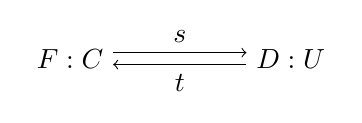
\begin{tikzpicture}[node distance=2.8cm, auto]
	
	\node (P) {$F : C$};
	\node(Q)[right of=P] {$D : U$};
	
	\draw[transform canvas={yshift=0.5ex},->] (P) --(Q) node[above,midway] {$s$};
	\draw[transform canvas={yshift=-0.5ex},->](Q) -- (P) node[below,midway] {$t$};
	
	\end{tikzpicture}
\end{center}

\bigskip

and a natural transformation:

\begin{center}
	$\eta : 1_{C} \rightarrow U \circ F$
\end{center}

that follows the diagrams:

	\bigskip

\begin{large}
	\begin{center}
		
		\begin{tikzcd}
			F(C) \arrow[dotted]{r}{g} 
			&D
		\end{tikzcd}
	\end{center}
\end{large}

\bigskip

\begin{large}
	\begin{center}
		\begin{tikzcd}
			C \arrow{r}{\eta_{C}} \arrow{rd}[swap]{f}
			&U(F(C)) \arrow{d}{U(g)}\\
			& U(D)
		\end{tikzcd}
	\end{center}
\end{large}

\bigskip

\end{mydefi}

In the above definition, $F$ is called the left adjoint, $U$ the right adjoint and $\eta$ is the unit of the adjunction. In the monoid example, the left adjoint is the free monoid generator and the right adjoint is the forgetful functor.

\section{Higher Categories}

In this section, we introduce only the concepts of higher category theory that will be necessary to prove our results in the next chapter. 

Previously in this chapter, we have said that sometimes the arrows between two objects do not form only a set, but a category instead. In that case, we have categories between every pair of objects. In this sense, we can think that we have added a new dimension to the category. Indeed, this process can continue. We can take a category, then a category between pair of objects and go even further, taking a category between pairs of objects of this inner category. This process can add infinitely many dimensions. When this process goes up to the infinity, we have an $\infty-groupoid$. 

Another important concept is the fact that sometimes the equalities of a category does not hold "on the nose", but only in a weak sense. For example, we have seen the difference between definitional and propositional equalities in type theory. In this theory, the equalities of a category induced by a type do not hold in the strict sense of definitional equalities, but only hold up to propositional equality, thus they are weak structures. In fact, weak structures are much more common in mathematics than strict ones. Thus, we are going to be interested in weak higher order categories.

Moreover, it is important to notice that we are going to limit the scope of this work to weak categories of the second order, called bicategories. Obtaining a weak $\infty$-groupoid would be a great achievement, but since it involves many highly complex concepts of higher category theory, trying to achieve this result would be unpractical.

With that said, we can finally define some basic concepts of higher category theory.

\subsection{Globular Sets}

The first important concept is globular set:

\begin{mydefi}[Globular Sets \cite{Tom}]
	Let $n \in \mathbb N$. A globular set $X$ is the following diagram of sets and functions:

\bigskip

\begin{center}
	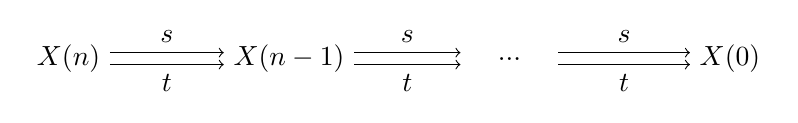
\begin{tikzpicture}[node distance=2.8cm, auto]
	
	\node (P) {$X(n)$};
	\node(Q)[right of=P] {$X(n-1)$};
	\node (R)[right of =Q] {$\quad ... \quad$};
	\node(S)[right of =R] {$X(0)$};
	
	\draw[transform canvas={yshift=0.5ex},->] (P) --(Q) node[above,midway] {$s$};
	\draw[transform canvas={yshift=-0.5ex},->](P) -- (Q) node[below,midway] {$t$};
	\draw[transform canvas={yshift=0.5ex},->] (Q) --(R) node[above,midway] {$s$};
	\draw[transform canvas={yshift=-0.5ex},->](Q) -- (R) node[below,midway] {$t$};
	\draw[transform canvas={yshift=0.5ex},->] (R) --(S) node[above,midway] {$s$};
	\draw[transform canvas={yshift=-0.5ex},->](R) -- (S) node[below,midway] {$t$};
	
	\end{tikzpicture}
\end{center}

\bigskip

The diagram must respect the following equations for any  $m \in \{2, . . . ., n\}$ and  $x\in X(m)$:

\begin{center}
	$s(s(x)) = s(t(x))$, \quad $t(s(x)) = t(t(x))$
\end{center}


The terms $x \in X(n)$ are called $n$-cells.

\end{mydefi}

\subsection{Horizontal Composition}

Given any globular set, a $0$-cell is simply an object and is represented by the following diagram:

\bigskip

\begin{center}
	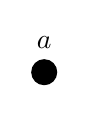
\begin{tikzpicture}[>=latex,
	every node/.style={auto},
	arrowstyle/.style={double,->,shorten <=3pt,shorten >=3pt},
	mydot/.style={circle,fill}]
	
	\coordinate[mydot,label=above:$a$](a)  at (0,0);
	\end{tikzpicture}
\end{center}
\bigskip

An $1$-cell is a morphism between objects, represented by:

\bigskip
\begin{center}
	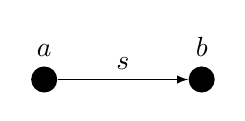
\begin{tikzpicture}[>=latex,
	every node/.style={auto},
	arrowstyle/.style={double,->,shorten <=3pt,shorten >=3pt},
	mydot/.style={circle,fill}]
	
	\coordinate[mydot,label=above:$a$](a)  at (0,0);
	\coordinate[mydot,label=above:$b$](b) at (2,0);
	
	\draw[->]   (a) to coordinate (s) node[] {$s$}    (b);
	
	\end{tikzpicture}
\end{center}
\bigskip

$2$-cells are morphisms between $1$-cells. Therefore, are represented by the following diagram:

\bigskip

\begin{center}
	
	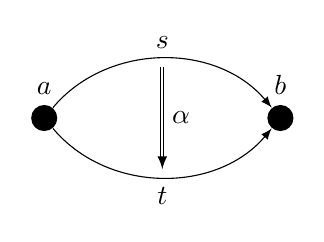
\begin{tikzpicture}[>=latex,
	every node/.style={auto},
	arrowstyle/.style={double,->,shorten <=3pt,shorten >=3pt},
	mydot/.style={circle,fill}]
	
	\coordinate[mydot,label=above:$a$](a)  at (0,0);
	\coordinate[mydot,label=above:$b$](b) at (3,0);
	
	\draw[->]   (a) to[bend left=50]  coordinate (s) node[]{$s$}          (b);
	\draw[->]   (a) to[bend right=50] coordinate (t) node[,swap]{$t$}    (b);
	
	\draw[arrowstyle] (s) to node[right]{$\alpha$} (t);
	\end{tikzpicture}	
	
\end{center}
\bigskip

Since a $2$-cell has a higher dimension that $1$-cells, it is possible to compose $2$-cells in two different ways. The first way is the traditional composition written as $\circ$. The diagram

\bigskip

\begin{equation*}
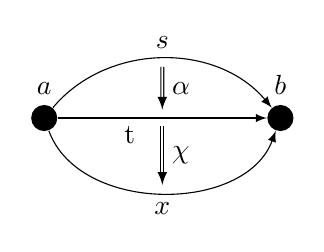
\begin{tikzpicture}[>=latex,
every node/.style={auto},
arrowstyle/.style={double,->,shorten <=3pt,shorten >=3pt},
mydot/.style={circle,fill}]

\coordinate[mydot,label=above:$a$](a)  at (0,0);
\coordinate[mydot,label=above:$b$](b) at (3,0);

\draw[->]   (a) to[bend left=50]  coordinate (s) node[]{$s$}          (b);
\draw[->]   (a) to coordinate (t) node[label={[label distance=-1cm]43:t}] {}    (b);
\draw[->]   (a) to[bend right=70]  coordinate (x) node[,swap]{$x$}          (b);

\draw[arrowstyle] (s) to node[right]{$\alpha$} (t);
\draw[arrowstyle] (t) to node[right]{$\chi$} (x);

\end{tikzpicture}
\end{equation*}

\bigskip

\noindent can be represented by:

\bigskip

\begin{equation*}
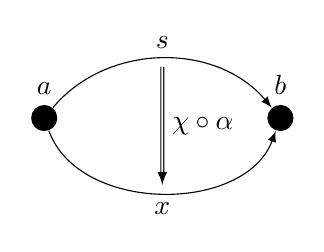
\begin{tikzpicture}[>=latex,
every node/.style={auto},
arrowstyle/.style={double,->,shorten <=3pt,shorten >=3pt},
mydot/.style={circle,fill}]

\coordinate[mydot,label=above:$a$](a)  at (0,0);
\coordinate[mydot,label=above:$b$](b) at (3,0);

\draw[->]   (a) to[bend left=50]  coordinate (s) node[]{$s$}          (b);
\draw[->]   (a) to[bend right=70]  coordinate (x) node[,swap]{$x$}          (b);

\draw[arrowstyle] (s) to node[right]{$\chi \circ \alpha$} (x);


\end{tikzpicture}
\end{equation*}

\bigskip

In a $2$-cell, the traditional composition is also known as vertical composition.  For $2$-cells, we have an additional composition written as $\circ_{h}$. It is called horizontal composition \cite{Tom}.  It is represented by transforming the following diagram 

\bigskip

\begin{equation*}
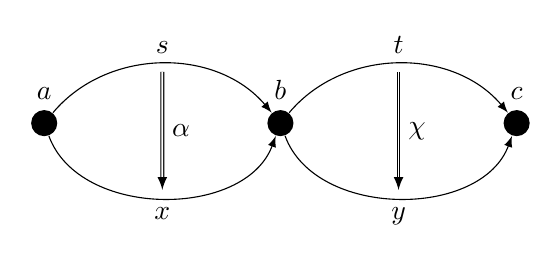
\begin{tikzpicture}[>=latex,
every node/.style={auto},
arrowstyle/.style={double,->,shorten <=3pt,shorten >=3pt},
mydot/.style={circle,fill}]

\coordinate[mydot,label=above:$a$](a)  at (0,0);
\coordinate[mydot,label=above:$b$](b) at (3,0);
\coordinate[mydot,label=above:$c$](c) at (6,0);

\draw[->]   (a) to[bend left=50]  coordinate (s) node[]{$s$}          (b);
\draw[->]   (a) to[bend right=70]  coordinate (x) node[,swap]{$x$}          (b);

\draw[->]   (b) to[bend left=50]  coordinate (t) node[]{$t$}          (c);
\draw[->]   (b) to[bend right=70]  coordinate (y) node[,swap]{$y$}          (c);

\draw[arrowstyle] (s) to node[right]{$\alpha$} (x);
\draw[arrowstyle] (t) to node[right]{$\chi$} (y);

\end{tikzpicture}
\end{equation*}

\bigskip

\noindent into the diagram:

\bigskip

\begin{equation*}
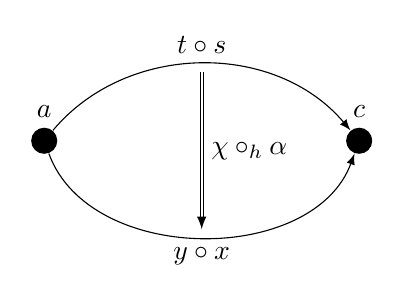
\begin{tikzpicture}[>=latex,
every node/.style={auto},
arrowstyle/.style={double,->,shorten <=3pt,shorten >=3pt},
mydot/.style={circle,fill}]

\coordinate[mydot,label=above:$a$](a)  at (0,0);
\coordinate[mydot,label=above:$c$](c) at (4,0);

\draw[->]   (a) to[bend left=50]  coordinate (s) node[]{$t \circ s$}          (c);
\draw[->]   (a) to[bend right=70]  coordinate (x) node[,swap]{$y \circ x$}          (c);

\draw[arrowstyle] (s) to node[right]{$\chi \circ_{h} \alpha$} (x);

\end{tikzpicture}
\end{equation*}

\bigskip

Thus, when one works with categories of order higher than $1$, one needs to take into account those new kind of compositions. In the case of $2$-categories, the $2$-cells will have those two compositions. Moreover, the horizontal composition must also respects associativity and the identity laws. Analogously, $3$-cells, in addition of the two compositions present in $2$-cells, has a third one. Indeed, a $n$-cell has $n$ compositions. Formally, $m$ compositions of a $m$-cell  $\in A(m)$ is represented by \cite{Tom}:

\begin{center}
	
	$A(m) \times_{A(p)} A(m) = \{ (x',x) \in A(m) \times A(m) \mid t^{m-p}(x) = s^{m-p}(x') \}$, with $p \leq m$
\end{center}

\subsection{Bicategories}

Bicategories are weak second order categories. They are defined as follows:

\begin{mydefi}[Bicategories \cite{leinster1}]
	
A bicategory $\Gamma$ is a structure with the following data and axioms:

\noindent Data:

\begin{itemize}
	
	\item Objects collection ob $\Gamma$ (Elements are $0$-cells $A, B, ...$)
	\item Categories $\Gamma(A,B)$ ($1$-cells $f, g, ...$ are the objects of those categories and arrows are  $2$-cells $\alpha, \beta, ...$)
	\item Functors:
	
	\begin{center}
		
		$c_{ABC} : \Gamma(B,C) \times \Gamma(A,B) \rightarrow \Gamma(A,C)$
		
		$(g,f) \rightarrow g \circ f = gf$
		
		$(\beta,\alpha) \rightarrow \beta \circ_{h} \alpha$\\
and $I_{A}: 1 \rightarrow \Gamma(A,A)$ (thus, $I_{A}$ is an $1$-cell $A \rightarrow A$)

	\end{center}



\item The following natural isomorphisms:


\begin{figure}[!htb]
	\centering
	\includegraphics[width=1\columnwidth]{images/naturaltransf.png}
\end{figure}

Thus, we have $2$-cells:

\begin{center}
	
	$a_{hgf}: (hg)f  \xrightarrow{\sim} h(gf)$
	
	$r_{f}: f \circ I_{A}  \xrightarrow{\sim} f$
	
	$l_{f}: I_{B} \circ f  \xrightarrow{\sim} f$
	
\end{center}

\end{itemize}

Axioms:

\noindent Consider the following configuration of $1$-cells

\bigskip
\begin{center}
	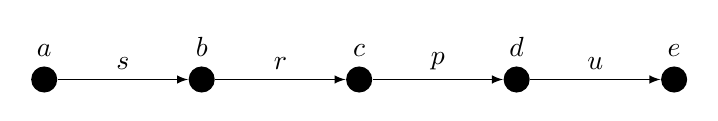
\begin{tikzpicture}[>=latex,
	every node/.style={auto},
	arrowstyle/.style={double,->,shorten <=3pt,shorten >=3pt},
	mydot/.style={circle,fill}]
	
	\coordinate[mydot,label=above:$a$](a)  at (0,0);
	\coordinate[mydot,label=above:$b$](b) at (2,0);
	\coordinate[mydot,label=above:$c$](c) at (4,0);
	\coordinate[mydot,label=above:$d$](d) at (6,0);
	\coordinate[mydot,label=above:$e$](e) at (8,0);
	
	\draw[->]   (a) to coordinate (s) node[] {$s$}    (b);
	\draw[->]   (b) to coordinate (r) node[] {$r$}    (c);
	\draw[->]   (c) to coordinate (p) node[] {$p$}    (d);
	\draw[->]   (d) to coordinate (u) node[] {$u$}    (e);
	
	
	\end{tikzpicture}
\end{center}

\bigskip

The following diagrams commute:

\bigskip

\begin{center}
	\begin{tikzpicture}[>=latex,
	every node/.style={auto},
	arrowstyle/.style={double,->,shorten <=3pt,shorten >=3pt},
	mydot/.style={circle,fill}]
	
	\coordinate[mydot,label=left:$((u\circ p) \circ r) \circ s$](a)  at (2,0);
	\coordinate[mydot,label=left:$(u \circ p) \circ (r \circ s)$](b) at (0,-3);
	\coordinate[mydot,label=right:$(u \circ(p \circ r)) \circ s$](c) at (5,0);
	\coordinate[mydot,label=right:$u \circ((p \circ r) \circ s) $](d) at (7,-3);
	\coordinate[mydot,label=below:$u \circ (p \circ (r \circ s))$](e) at (3.5,-6);
	
	\draw[->]   (a) to coordinate (s) node[,swap] {$a$}    (b);
	\draw[->]   (a) to coordinate (t) node[,swap] {$a \circ_{h} 1$}    (c);
	\draw[->]   (c) to coordinate (x) node[] {$a$}    (d);
	\draw[->]   (b) to coordinate (y) node[,swap] {$a$}    (e);
	\draw[->]   (d) to coordinate (z) node[] {$1 \circ_{h} a$}    (e);
	\end{tikzpicture}
\bigskip

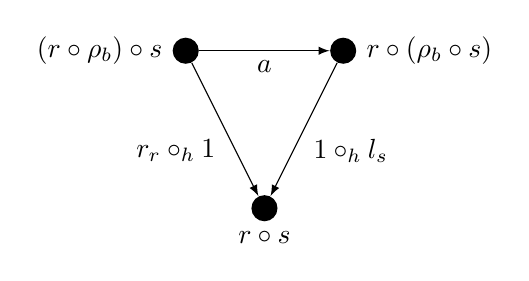
\begin{tikzpicture}[>=latex,
every node/.style={auto},
arrowstyle/.style={double,->,shorten <=3pt,shorten >=3pt},
mydot/.style={circle,fill}]

\coordinate[mydot,label=left:$(r \circ \rho_{b}) \circ s$](a)  at (0,0);
\coordinate[mydot,label=right:$r \circ (\rho_{b} \circ s)$](b) at (2,0);
\coordinate[mydot,label=below:$r \circ s$](c) at (1,-2);

\draw[->]   (a) to coordinate (s) node[,swap] {$a$}    (b);
\draw[->]   (a) to coordinate (t) node[,swap] {$r_{r} \circ_{h} 1$}    (c);
\draw[->]   (b) to coordinate (x) node[] {$ 1 \circ_{h} l_{s}$}    (c);
\end{tikzpicture}
\end{center}

\bigskip

\end{mydefi}

In the literature of higher order category theory, the axioms of a weak higher order category are called coherence laws \cite{Tom}.

\section{Conclusion}

In this chapter, we have seen the basic concepts of category theory. Most will play an important role in the next chapter. The concepts of isomorphism and groupoid, for instance, will be the base for mathematical model for computational paths. We have also seen concepts of higher category theory, since in the sequel we are going to show that computational paths forms a higher structure. 

